\documentclass[11pt]{article}
\usepackage{amsmath}
\usepackage{graphicx}
\usepackage{hyperref}

\begin{document}

\title{Assignment 2: Cost-Sensitive Regression}
\author{Team Members: CS21BTECH11060, MA22BTECH11015, AI22BTECH11020}
\maketitle

\section{Introduction}
Fraud detection in financial transactions is a challenging task due to the high cost associated with misclassifications, particularly false negatives. In this work, we compare a standard (vanilla) logistic regression model with a cost-sensitive logistic regression model based on Bahnsen's approach. The comparison is performed on a dataset containing financial transaction features, class labels, and a cost associated with misclassification. The goal is to understand how varying the decision threshold (offset) affects the cost, and to analyze the convergence of the cost-sensitive method.

\section{Dataset Description}
The dataset (\texttt{costsensitiveregression.csv}) contains 13 columns:
\begin{itemize}
    \item The first 11 columns represent various features of financial transactions.
    \item The 12th column is the binary class label (0 for non-fraudulent, 1 for fraudulent).
    \item The 13th column gives the false negative cost (cost incurred if a fraudulent transaction is misclassified as non-fraudulent).
\end{itemize}
In our preprocessing, we reorder the columns so that the class label becomes the first column and the cost column (named \texttt{FNC}) is separated from the feature set. The data is then split into training and testing sets.

\section{Methodology}
Two logistic regression models are compared:
\begin{enumerate}
    \item \textbf{Vanilla Logistic Regression:} A standard logistic regression model is trained using scikit-learn. The decision function (logits) is adjusted by an offset before computing probabilities. The cost is defined as (100 - accuracy) for the sake of comparison.
    \item \textbf{Cost-Sensitive Logistic Regression (Bahnsen's Approach):} A genetic algorithm optimizes a logistic regression model using a cost-sensitive loss function (Bahnsen cost). The cost function is defined as:
    \[
    J(\theta) = -\frac{1}{m} \sum_{i=1}^{m} \Big[ y^{(i)} (c_{tp}\,h_{\theta}(x^{(i)}) + c_{fn}\,(1-h_{\theta}(x^{(i)})) ) + (1-y^{(i)}) (c_{fp}\,h_{\theta}(x^{(i)}) + c_{tn}\,(1-h_{\theta}(x^{(i)})) ) \Big]
    \]
    where \(c_{tp} = c_{fp} = 6\) and \(c_{tn} = 0\). The false negative cost is row-dependent.
\end{enumerate}
For both models, we vary an offset (added to the model’s logits) and evaluate the corresponding cost. In addition, for the Bahnsen approach we also monitor the cost evolution over the iterations of the genetic algorithm.

\section{Results}
The following figures illustrate the impact of varying the offset on the cost for both approaches, and the convergence behavior of the Bahnsen model.

\subsection{Vanilla Logistic Regression: Cost vs. Offset}
Figure~\ref{fig:vanilla_offset} shows the cost (defined as 100 minus the accuracy) for the vanilla model as the offset is varied from -2 to 2.
\begin{figure}
    \centering
    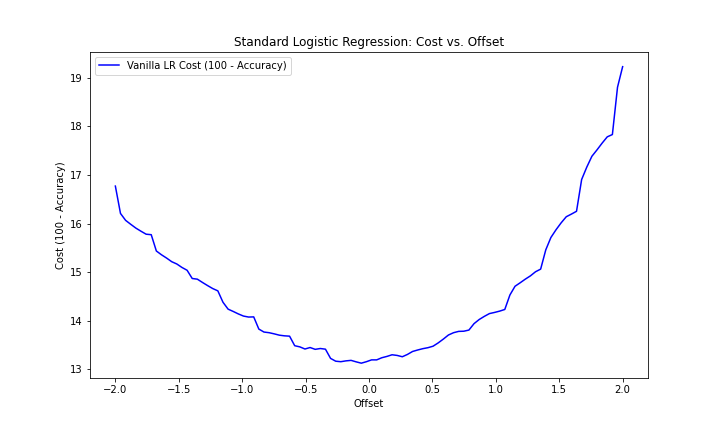
\includegraphics[width=0.8\textwidth]{../vanilla_lr_cost_vs_offset.png}
    \caption{Vanilla Logistic Regression: Cost vs. Offset}
    \label{fig:vanilla_offset}
\end{figure}

\subsection{Bahnsen Logistic Regression: Cost vs. Offset}
Figure~\ref{fig:bahnsen_offset} shows the cost computed using Bahnsen's cost function for various offsets.
\begin{figure}
    \centering
    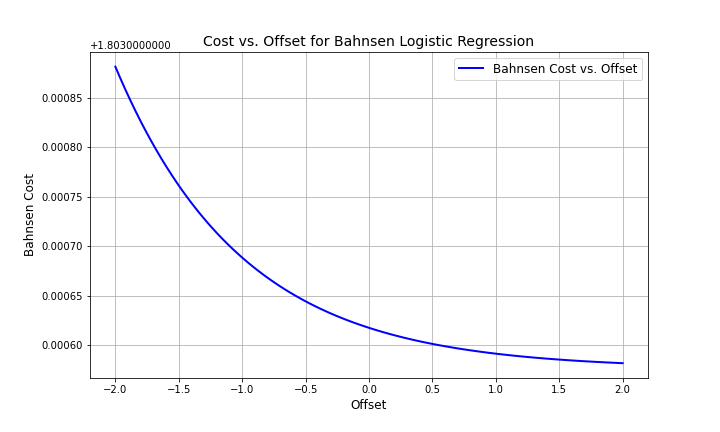
\includegraphics[width=0.8\textwidth]{../bahnsen_cost_vs_offset.png}
    \caption{Bahnsen Logistic Regression: Cost vs. Offset}
    \label{fig:bahnsen_offset}
\end{figure}

\subsection{Bahnsen Logistic Regression: Cost vs. Iterations}
Figure~\ref{fig:bahnsen_iterations} presents the evolution of the cost (as computed on the training set) over the iterations of the genetic algorithm used to optimize the Bahnsen model.
\begin{figure}
    \centering
    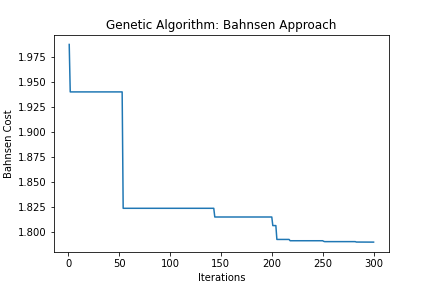
\includegraphics[width=0.8\textwidth]{../bahnsen_plot.png}
    \caption{Bahnsen Logistic Regression: Cost vs. Iterations}
    \label{fig:bahnsen_iterations}
\end{figure}

\section{Comparison and Analysis}
\begin{itemize}
    \item \textbf{Offset Sensitivity:} The vanilla model exhibits a cost that reaches a minimum near an offset of 0.5, while the cost-sensitive model (Bahnsen) shows a different trend due to the higher penalty for false negatives.
    \item \textbf{Cost Convergence:} The cost vs. iterations plot for the Bahnsen approach indicates that the genetic algorithm is able to steadily reduce the cost over time, demonstrating convergence.
    \item \textbf{Model Suitability:} In fraud detection scenarios where false negatives are significantly more expensive than false positives, the Bahnsen approach provides a better framework by incorporating misclassification costs directly into the loss function.
\end{itemize}

\section{Conclusion}
This report compared the performance of standard logistic regression with a cost-sensitive model based on Bahnsen's approach. The experiments reveal that the cost-sensitive model is more adept at handling the asymmetric costs of misclassification inherent in fraud detection, as evidenced by its distinct offset behavior and cost convergence pattern. Future work could further refine the optimization procedure and explore alternative cost functions.

\end{document}